\setcounter{chapter}{1}
\chapter*{Second year report}
\chaptermark{Chapter1}
\section{Introduction}
The work done in the first part of the second year of this phd program consisted of a determination of the CP-even fraction of the decay of the D meson into 4 pions. The CP-even fraction of the decay was determined using correlated \D meson pairs produced at the lepton collider CESR and reconstructed by the CLEO-c detector. The results of this analysis have been published are now used by the Oxford group to measure the CKM gamma angle using LHCb data. \\
The last month of work was used towards producing an alignment for the RICH detectors in the LHCb experiment for RunII.\\
\\
Unless otherwise stated all activities described in this report were performed by the author.\\

\section{Determining the CP-even fraction of $\D \rightarrow 4\pi $}
\subsection{Short theory}
The simplest way of determining the CP-even fraction of a decay using correlated pairs is by measuring the rate of events against decays with definitive CP-eigenstates. This part of the analysis was performed by the Oxford group.\\
Another way of determining the CP-even fraction is by reconstructing it against a decay which strong phase difference in different bins of phasespace has been determined previously. The decay used here is $\D \rightarrow \KsPiPi$ and $\D \rightarrow \KlPiPi$.\\
The CP-even fraction $F_+^{4\pi}$ of $ 4\pi$ can be determined through the evaluation of
\begin{equation}
M^{\KsPiPi}_i = h_{\KsPiPi} (T^{\KsPiPi}_i + T^{\KsPiPi}_{-i} - 2 \, c_i  \sqrt{T^{\KsPiPi}_i T^{\KsPiPi}_{-i}} \ (2 F_+^{4\pi} -1))
\end{equation}
and
\begin{equation}
M^{\KlPiPi}_i =  h_{\KlPiPi} (T^{\KlPiPi}_i + T^{\KlPiPi}_{-i} + 2 \, c'_i  \sqrt{T^{\KlPiPi}_i T^{\KlPiPi}_{-i}} \ (2 F_+^{4\pi} -1))
\end{equation}
where the $M_i$ denote the number of events in bin $i$ of the \KsPiPi / \KlPiPi Dalitz-Plot tagged against \4Pi , the $T_i$ the relative amount of events in bin $i$ of flavour-tagged \KsPiPi / \KlPiPi Dalitz-Plot and the $h$ are normalisation factors.\\
By summing over the bins $i$ and $-i$ these expressions become
\begin{equation}
MM^{\KsPiPi}_i = M^{\KsPiPi}_i + M^{\KsPiPi}_{i} =2\cdot h_{\KsPiPi} (T^{\KsPiPi}_i + T^{\KsPiPi}_{-i} - 2 \, c_i  \sqrt{T^{\KsPiPi}_i T^{\KsPiPi}_{-i}} \ (2 F_+^{4\pi} -1))
\end{equation}
and
\begin{equation}
MM^{\KlPiPi}_i = M^{\KlPiPi}_i + M^{\KlPiPi}_{-i} = 2\cdot h_{\KlPiPi} (T^{\KlPiPi}_i + T^{\KlPiPi}_{-i} + 2 \, c'_i  \sqrt{T^{\KlPiPi}_i T^{\KlPiPi}_{-i}} \ (2 F_+^{4\pi} -1))
\end{equation}
The following report summarised how the values for $MM^{\KsPiPi}_i$ and $MM^{\KlPiPi}_i$ are determined.\\


\subsection{Binned \KsPiPi / \KlPiPi vs \4Pi yields}

The values for $MM_i(\KsPiPi)$ are obtained by counting the number of \KsPiPi / \KlPiPi vs. \4Pi events, subtracting the bkg in the sample and then correcting for different signal reconstruction and selection efficiencies in the different bins of the \KsPiPi / \KlPiPi Dalitz-Plot. The contributions to the yields for the \KsPiPi tag are listed below:
\begin{equation}
MM^{\KsPiPi}_i = (N_i^{meas} - B_i^{peak} - B_i^{flat})/ \epsilon_i
\end{equation}
\begin{itemize}
\item $MM^{\KsPiPi}_i$ : absolute number of \4Pi vs \KsPiPi events in bin i. This is the quantity that enters the fit for $F_+$.\\
\item $N_i^{meas}$ : total number of reconstructed and selected events in bin i. \\
\item $B_i^{peak}$ : number of reconstructed and selected peaking bkg. events in bin i. The only peaking bkg. expected is \KsPiPi vs \KsPiPi where on of the \KsPiPi decays is reconstructed as a \4Pi . \\
\item $B_i^{flat}$ : number of reconstructed and selected flat bkg. events in bin i.\\
\item $\epsilon_i$ : reconstruction and selection efficiency for \4Pi vs \KsPiPi events in bin i. \\
\end{itemize}

The values for $MM^{\KlPiPi}_i$ are obtained using:
\begin{equation}
MM^{\KlPiPi}_i = (N_i^{meas} - B_i^{peak} - B_i^{flat} - B_i^{cont})/ \epsilon_i
\end{equation}
\begin{itemize}
\item $MM^{\KlPiPi}_i$ : absolute number of \4Pi vs \KlPiPi events in bin i. This is the quantity that enters the fit for $F_+$.\\
\item $N_i^{meas}$ : total number of reconstructed and selected events in bin i. \\
\item $B_i^{peak}$ : number of reconstructed and selected peaking bkg. events in bin i. The two peaking bkgs considered in this case are \KlPiPi vs \KsPiPi where the \KsPiPi is reconstructed as \4Pi (8\% of the events in the signal window) and \KsPiPi vs \4Pi where the \KS is not reconstructed (1.9\% of the events in the signal window). \\
\item $B_i^{flat}$ : number of reconstructed and selected flat bkg. events in bin i.\\
\item $B_i^{cont}$ : number of reconstructed and selected continuum bkg. events in bin i.\\
\item $\epsilon_i$ : reconstruction and selection efficiency for \4Pi vs \KlPiPi events in bin i. \\
\end{itemize}
The contributions for the \KlPiPi tag have another component, which is the continuum bkg. This bkg does not appear in the \KsPiPi tag because in this tag requires 4 pions to be reconstructed while in the \KlPiPi case only 2 pions are reconstructed.
\\
The distribution of reconstructed \KsPiPi / \KlPiPi vs \4Pi events in the phasespace of the tag can be seen in Figure \ref{ps}.

\begin{figure}[!h]
\begin{center}
\subfigure{ 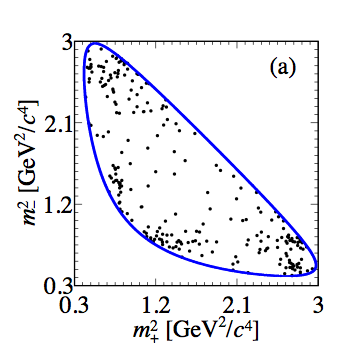
\includegraphics[width=0.48 \textwidth] {KsPiPips.png}}
\subfigure{ 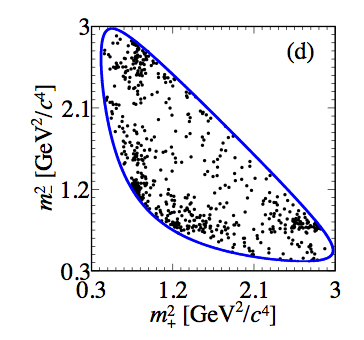
\includegraphics[width=0.48 \textwidth] {KlPiPips.png}}
\end{center}
\caption{\textit{Dalitz-plot distributions for \KsPiPi (left) and \KlPiPi (right) reconstructed against 4\Pi.}}
\label{ps}
\end{figure}

\subsubsection{Determination of number of flat and continuum background events}
\label{sec:flat}
The total number of flat bkg events is determined using a combination of sidebands and extrapolated to the signal region. As the name suggest, the flat background is distributed evenly over the \KsPiPi phasespace. Therefore the distribution across the different \KsPiPi bins is used according to the area of each bin.\\
The same is true for the continuum bkg, only that the total number of continuum bkg events was determined using the continuum MC sample produced by CLEO-c and scaling according to the luminosity of the data sample.\\

\subsubsection{Determination of peaking bkg events}
The total number of peaking bkg events was determined by scaling their contribution in the generic MC sample to the data sample. The distribution of those events over the bins of the \KsPiPi / \KlPiPi phasespace was determined using a combination of data-driven and MC-driven techniques.\\
  
\subsubsection{Determination of the signal efficiency}
The signal efficiency of both the \KsPiPi and the \KlPiPi tags were determined using a signal MC sample of 250k events.\\


\subsection{Fit for $F_+(4\pi)$}
\subsubsection{Input from former analyses}
The given values for $K'_i$ obtained from Table 1 of \texttt{arXiv:1210.939} contain effects from charm-mixing that cancel in our case. The factors $T_i$ without mixing are archived by numerically solving the system of equations:
\begin{equation}
K'_i = T_i + \sqrt{T_i T_{-i}} (y c_i + x s_i)
\end{equation}
where $x$ and $y$ charm-mixing parameters. The fit also takes into account that the sum over the $T_i$ should be one by fixing  $T_1 = 1 - \sum_{i \neq 1} T_i$. The values for $x$ and $y$ are take from the latest HFAG results ($x = (0.63 \pm 0.19)\%$, $y = (0.75 \pm 0.12)\% $) and the values for $c_i$ and $s_i$ are taken from \texttt{arXiv:1010.2817}. In the fit all input variables are Gaussian constraint and the correlation between $c_i$ and $s_i$ are taken into account.\\
\\
The fractional flavour-tagged \KlPiPi yields are taken from Sean Brisbane's thesis (Section 3., Table 3.14).\\

\subsubsection{Results $F_+$ }
A fit for $F_+$ is performed for the default signal results, for the results with stat. error only.\\
In order to determine the effect of the systematic uncertainties - most of which come for the estimation of bkg events - the each systematic uncertainty is separately added to the statistic uncertainty and the fit is performed again.\\
Listing the statistical error and the systematic error from the Dalitz plot acceptance separately this results in $F_+ = 0.737 \pm 0.049 \pm 0.024$ where the first error is statistical and the second one systematic. These results are in very good agreement with the result from the CP-eigenstate analysis which yielded a value of $F_+ = 0.754 \pm 0.031 \pm 0.021$.
\clearpage
\begin{figure}[!h]
\begin{center}
\subfigure{ 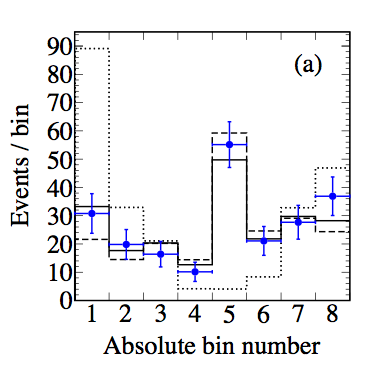
\includegraphics[width=0.48 \textwidth] {FKsPiPi.png}}
\subfigure{ 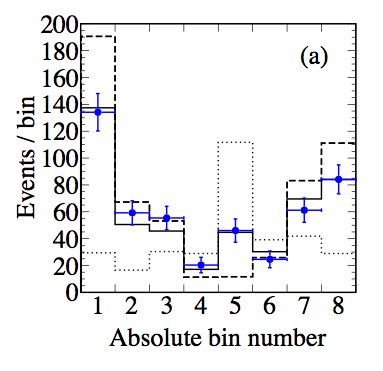
\includegraphics[width=0.48 \textwidth] {FKlPiPi.png}}
\end{center}
\caption{\textit{Distribution of signal yields per bin for \KsPiPi (left) and \KlPiPi (right). Red: data, solid line: fit results, dotted line: values for $F_+$=0, dashed line: values for $F_+$=1.0.}}
\end{figure}


\section{RICH alignment}
The work on the RICH alignment for the LHCb detector consists mostly of making the existing alignment code work and producing an alignment on the data taken in the last days.\\
Additionally work on the ONLINE RICH alignment is ongoing which - amongst other things - consists of rewriting the existing alignment script in a way that is compatible with the Finite State Machine system under which the entire online framework operates.\\

\section{Future work}
The work for the next year includes the following steps
\begin{itemize}
\item finalize the work on the RICH alignment by producing a functioning and hopefully stable online alignment 
\item perform a $c_i$ and $s_i$ measurement for \DTo4Pi on CLEO-c data and publish this
\item if there is still time left in the year start working on the $\gamma$ measurement at LHCb
\end{itemize}

\newpage

\section{Thesis outline}
\begin{itemize}
\item \textbf{Chapter 1: Introduction and overview} (5 pages)\\
\item \textbf{Chapter 2: Theory} (15 pages)\\
	Includes the Standard Model with a special emphasis on CP violation and the CKM matrix; Amplitude-model-independent methods to measure $\gamma$ in \B $\rightarrow$ \D \kaon decays, binned analysis measuring/using $c_i$ and $s_i$ and global analysis measuring/using the CP even fraction $F_+$.
\item \textbf{Chapter 3: Detectors} (20 pages)\\
CLEO-c detector and LHCb detector with special emphasis on the RICH system of the latter.\\
\item \textbf{Chapter 4: Real-time RICH alignment at LHCb} (20 pages)\\
\item \textbf{Chapter 5: CLEO-c analyses} (40 - 50 pages)\\
Measuring the CP even fraction of \D $\rightarrow$ 4\pion and measuring $c_i$ and $s_i$.\\
\item \textbf{Chapter 6: LHCb analysis} (30 - 40 pages)\\
Measuring $\gamma$ with \B $\rightarrow$ \D \kaon , \D $\rightarrow$ 4\pion .
\item \textbf{Chapter 7: Conclusion }(5 pages)
\end{itemize}

